% !TeX encoding = UTF-8
% !TeX program = pdflatex
% !TeX spellcheck = it_IT

\documentclass[binding=0.6cm,TFA]{sapthesis}

\usepackage{microtype}
\usepackage[italian]{babel}
\usepackage[utf8]{inputenc}
\usepackage[hidelinks]{hyperref}
\usepackage{setspace}
\usepackage[Algoritmo]{algorithm}
\usepackage{algorithmic}
\usepackage{graphicx}
\usepackage{listings}
\usepackage{xcolor}
\lstset { %
    language=C++,
    backgroundcolor=\color{black!5}, % set backgroundcolor
    basicstyle=\footnotesize,% basic font setting
}
\usepackage[chapter]{minted}

\renewcommand\listingscaption{Codice}

\onehalfspacing
\graphicspath{ {assets/} }

\hypersetup{pdftitle={Green IoT: Design e valutazione delle prestazioni di protocolli per sistemi IoT dotati di wake up radio},pdfauthor={Leonardo Emili}}

\title{Green IoT: Design e valutazione delle prestazioni di protocolli per sistemi IoT dotati di wake up radio}
\author{Leonardo Emili}
\IDnumber{1802989}
\course{Informatica L-31}
\courseorganizer{Facoltà di Ingegneria dell'informazione, informatica e statistica}
\AcademicYear{2019/2020}
\copyyear{2020}
\advisor{Prof. Chiara Petrioli}
\tutor{Dr. Georgia Koutsandria}
\tutorcoord{Prof. Chiara Petrioli}
\tutorcoord{Dr. Georgia Koutsandria}
\authoremail{emili.1802989@studenti.uniroma1.it}

\begin{document}
\large

\frontmatter
\maketitle

\tableofcontents

\mainmatter
\chapter{Introduzione}

Nell'ultimo decennio abbiamo assistito ad uno sviluppo portentoso del settore dell'Internet of Things che ha contribuito alla diffusione
di un enorme numero di dispositivi wireless. Il numero di questi dispositivi ha registrato crescite costanti negli anni e loro applicazioni sono ormai infinite.
Essi trovano impiego in ambito domestico dove realizzano l'automatizzazione dei compiti quotidiani, in quello sanitario in cui monitorano lo stato di salute
dei pazienti e in ambito sottomarino dove gli obbiettivi spaziano da quello di realizzare campionamenti di dati sino a creare vaste reti di comunicazione sottomarine.
L'immissione di questo enorme contingente di dati nella rete ha reso possibili nuove interpretazioni e lo sviluppo di soluzioni che puntano a
migliorare la qualità della vita delle persone, anche in quei settori noti esser di difficile comprensione. Ad esempio, l'impiego di sensori IoT in ambito di
monitoraggio del crosta terrestre ha reso disponibili informazioni fino a prima sconosciute sulla presenza di terremoti e tsunami, migliorando radicalmente
la nostra percezione degli eventi sismici nel mondo.\\

Con lo sviluppo massivo dell'IoT nuove sfide sono emerse a minare la solidità degli approcci usati. Attualmente le soluzioni impiegate nello sviluppo
dei dispositivi wireless puntano a realizzare comunicazioni con basse latenze e che siano altamente efficienti in termini energetici. In ambito di ricerca,
lo stato corrente dell'arte punta a realizzare tecnologie hardware e software che implementino questo binomio. Un particolare
settore dell'IoT si occupa di realizzare vaste reti di nodi sensori interconnessi, note come \emph{Wireless Sensor Networks},
che realizzano una comunicazione wireless con consumi minimi al fine di prolungare i tempi di servizio dell'intera rete. In questo caso,
le principali problematiche sono chiaramente settoriali e sono identificate dallo specifico campo di applicazione: come la richiesta di tecnologie
altamente performanti per i monitoraggio clinici oppure di altre che garantiscano elevate lifetime nel caso di sensori ambientali. Tuttavia esistono
problematiche comuni a queste tipologie di reti, ad esempio spesso si richiede che l'intera rete sia connessa e che tutti i nodi siano,
anche parzialmente, a conoscenza della topologia della rete. Nel caso, si richiede l'impiego di protocolli che ne prevedano il
costante aggiornamento e favoriscano una comunicazione efficiente. Inoltre, in queste reti la principale fonte di consumo energetico risiede
nella comunicazione e nell'attesa che la precede, è quindi di vitale importanza prevedere che i nodi della rete siano
oggetto di scaricamento delle batterie che li alimentano. Infatti, la morte prematura di un nodo può spesso avere conseguenze più grandi della semplice
disconnessione dello stesso, poichè frequentemente si tratta di reti \emph{multi-hop} che realizzano la comunicazione passando attraverso nodi intermedi, si può
verificare perfino la disconnessione dell'intera rete.\\

Nel seguito verranno descritte le principali problematiche che motivano ricerca di nuove idee per la costruzione di protocolli di rete efficienti.
Nel capitolo seguente analizzeremo lo scenario di riferimento e le principali considerazioni che nel tempo sono state adottate e che ad oggi
definiscono il panorama delle Wireless Sensor Networks.\\

Nel \textbf{Capitolo 3} verrà presentato uno specifico protocollo di rete per sistemi IoT: il protocollo GREEN-WUP. In questo lavoro ci concentreremo sullo
studio dei principi che regolano il design dei protocolli di rete e sulla loro applicazione in riferimento al protocollo in questione. Analizzeremo
in dettaglio il comportamento del protocollo e le sue caratteristiche. Verranno inoltre presentati i suoi principali vantaggi ed il suo comportamento
di fronte a problematiche comuni ai protocolli di comunicazione.\\

Nel \textbf{Capitolo 4} verrà presentata una variante del protocollo originale che punta a risolvere le problematiche osservate nel capitolo precedente. Le
modifiche apportate saranno descritte in dettaglio sia a livello teorico che a livello di implementazione all'interno di Castalia che è
il simulatore utilizzato e a cui faremo diffusamente riferimento all'interno di questa relazione. In particolare, tutto il codice
a cui si fa riferimento in questo documento sono stati testati mediante una versione particolare del framework \emph{GreenCastalia}
che supporta \emph{wake up radios} e \emph{energy harvesting}.\\

Nel \textbf{Capitolo 5} saranno analizzate le prestazioni della variante proposta e quelle del protocollo originale. In particolare, verranno mostrati i
comportamenti di entrambe le implementazioni all'interno di uno stesso ambiente reale ed infine nel Capitolo 6 trarremo le conclusioni di quanto osservato.

\let\cleardoublepage    % probably not a good decision
\clearpage
\let\cleardoublepage\clearpage  % restore changes

\chapter{Scenario di riferimento}

Sino a qualche anno fa, la principale tendenza nello sviluppo di soluzioni ai problemi menzionati nel Capitolo 1 consisteva nell'introduzione di cicli di attività
dei nodi. Il cosiddetto \emph{duty cycling}, definito come la frazione di tempo in cui un nodo è attivo, aveva come obbettivo quello di minimizzare i momenti
in cui i nodi sensori sono accessi senza alcun processamento di dati attivo. Seppur questo approccio permetta di prolungare la durata della vita della rete,
incrementa in maniera considerevole i ritardi nelle comunicazioni, dal momento che queste possono avvenire solamente all'interno delle finestre di attività
delle coppie dei nodi coinvolti. Tuttavia l'utilizzo del duty cycling non permette di risolvere tutti i problemi in quanto le comunicazioni possono ancora
avvenire nei momenti di inattivà dei nodi. Dualmente, esistono ancora i periodi di tempo in cui i nodi consumano energia pur non ricevendo o inviando dati.\\


In questo panorama vengono introdotte le \emph{wake up radios}, in grado di abbattere i consumi energetici mantenendo bassi i ritardi nelle comunicazioni.
La principale differenza rispetto all'approccio tradizionale consiste nell'introdurre un'antenna secondaria per i soli messaggi di wake-up costantemente
attiva. La nuova antenna è progettata per avere di dimensioni ridotte e consumi energetici nettamente inferiori rispetto a quelli della radio principale.
Al momento della ricezione di un messaggio di wake-up è possibile attivarla e ricevere il pacchetto dati. Di fatto questa tecnologia implementa uno schema
di comunicazione \emph{on demand}: un nodo può inviare un pacchetto dati ad un nodo dormiente semplicemente  posticipandone l'invio a quello di una sequenza
di wake-up che, svegliando il ricevente, lo abilita alla ricezione. In questo modo i nodi possono rimanere attivi per il solo tempo minimo necessario a
svolgere l'attività richiesta e lasciare spenta la radio principale nel tempo rimanente. Dal punto vista energetico questo approccio è altamente efficiente
e non richiede alcuna forma di sincronizzazione che è generalmente non desiderata in quanto implicitamente introduce overhead dovuto alla gestione di timer
aggiuntivi.\\

Più recentemente la tendenza è quella di equipaggiare i nodi sensori, dotati di wake up radios, con moduli per l'\emph{energy harvesting} come ulteriore
supporto energetico alla loro durata di attività. In particolare, i nodi sono in grado di utilizzare l'energia fornita dalle pile elettriche di cui sono
forniti e di derivarne nuova mediante turbine eoliche, pannelli solari e generatori termoelettrici di cui sono equipaggiati. La ricerca ha dimostrato che
l'impiego di nodi dotati di energy harvesting \cite{energy-harvesting-paper} e che sono abilitati alle wake up radios \cite{wake-up-radios-paper} ha
portato notevoli incrementi nelle performance delle Wireless Sensor Networks.\\

Inoltre, l'innovativa tecnologia delle wake up radios può essere combinata con il cosiddetto \emph{semantic addressing}. L'idea in questo caso è di limitare
ad un sottoinsieme di nodi la ricezione di una sequenza di wake up, evitando quindi che questa sia recepita da tutti i nodi presenti all'interno
del range di comunicazione. Il principio fondante è quello di scegliere una o più opportune sequenze di wake up e di assegnarle ad un certo
sottoinsieme di nodi della rete. A meno di errori di interpretazione della sequenza di wake up, al momento della ricezione tutti e soli e nodi desiderati
saranno svegliati. In questo scenario, i consumi energetici risultano essere ulteriormente ridotti poichè viene virtualmente azzerato il numero dei nodi
che sono riattivati a seguito di sequenze di wake up non a loro destinate ma che si trovano all'interno del loro range.\\

Questo lavoro si concentra sullo studio di protocolli delle cosiddette \emph{green wireless sensor network}, ovverosia di quei protocolli che si basano
sulle tecnologie sopra esposte e che implementano la comunicazione tra nodi minimizzandone gli sprechi energetici al fine di massimizzare
i tempi di attività e il corretto funzionamento delle comunicazioni all'interno delle reti. Nella letteratura scientifica
sono presenti molti protocolli di questo tipo (es. CTP-WUR, GREENROUTES, WHARP) e ciascuno di loro punta a risolvere diverse problematiche.
Nel seguito verrà analizzato in dettaglio il comportamento del protocollo GREEN-WUP che utilizza energy harvesting e wake up radio per realizzare
un'opportuna scelta del percorso da seguire per permettere la ricezione dati da parte del sink node.\\

\chapter{Il protocollo GREEN-WUP}

\section{Descrizione del protocollo}

Il protocollo GREEN-WUP si inserisce nel contesto dei protocolli delle \emph{green wireless sensor network} e pone tra i suoi principali obiettivi
la massima efficienza energetica della rete. Esso impiega le tecnologie di wake up radio, energy harvesting e semantic addressing. Inoltre, è
di tipo \emph{converge casting} ed è basato sull'assegnazione di hop count a ciascun nodo per poter distribuire i pacchetti dati
all'interno della rete.\\

L'approccio tradizionale dei protocolli di rete prevede due fasi principali: in primo luogo avviene la fase di \emph{interest dissemination} dove si
definisce la topologia della rete da rispettare affinchè i nodi realizzino un corretto flusso di scambio dati; successivamente si assume che gli
indirizzi di wake up siano stati assegnati e si procede con lo scambio di dati che è governato da sequenze di wake up che vengono utilizzate per
risvegliare i nodi della rete. Nel caso specifico di GREEN-WUP la fase di interest dissemination non viene eseguita per motivi di efficienza
e gli hop count vengono determinati indirettamente prima ancora dell'inizio della simulazione. Per ragioni completezza in questo lavoro verrà
mostrata sia alla versione originale di GREEN-WUP che non comprende la fase di interest dissemination che una versione che la utilizza per
il calcolo degli hop count dei nodi della rete.\\

In GREEN-WUP ciascun nodo è fornito di una coppia di indirizzi di wake up. Si tratta infatti di un primo indirizzo che identifica univocamente
il nodo nella rete e rimane invariato nel tempo e di un altro che è mutabile nel tempo ed è definito a partire dallo stato corrente del nodo.
Quest'ultimo indirizzo di wake up è definito da una sequenza $w=w_{h}w_{e}$ della lunghezza di 8 bit, dove $w_{h}$ rappresenta il valore di hop
count $h$ del nodo in questione, $w_{e}$ invece rappresenta la sua attuale classe energetica. In particolare, ciascun nodo considera
l'energia disponibile come quella rimamente nelle batterie assieme a quella derivata da sorgenti esterne. In definitiva, la codifica del suffisso
$w_{e}$ viene calcolata a partire dalla discretizzazione in $k$ classi della disponibilità energetica di un nodo, dove $k$ rappresenta il
numero delle classi disponibili. Si noti come quest'ultimo indirizzo venga periodicamente aggiornato per riflettere la disponibilità
energetica del nodo nel tempo. Questa idea realizza il principio del semantic addressing poiché in questo scenario è possibile far riferimento
ad un sottoinsieme di nodi della rete a partire dai loro valori di hop count e da quello della classe energetica. \\

%image source: https://www.researchgate.net/figure/Topology-of-wireless-sensor-network-and-hop-count-of-sensors_fig7_285956270
\begin{figure}
    \begin{center}
        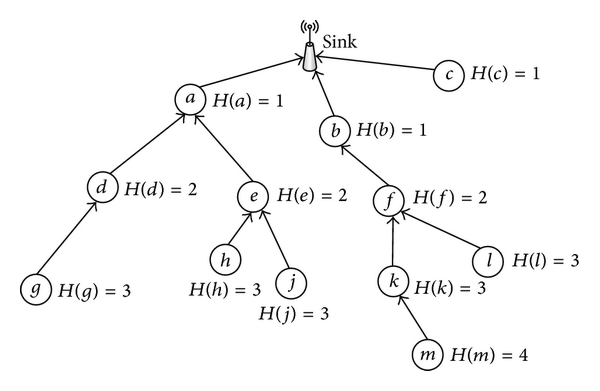
\includegraphics[scale=1.7]{hop-count-algorithm.png}
        \caption{Topologia della rete a seguito dell'assegnazione degli hop count.}
    \end{center}
\end{figure}

Nel momento in cui un nodo deve inviare un pacchetto dati può farlo seguendo degli step fondamentali di seguito descritti.
La prima fase consiste nell'instaurare una comunicazione con i nodi elegibili alla ritrasmissione del pacchetto: il suddetto nodo sensore
entra in uno stato di ricerca di un nodo che si farà carico della sua richiesta di ritrasmissione. La ricerca si considera conclusa
nel momento in cui viene selezionato un nodo tra quelli disponibili come nodo intermediario tra il nodo che invia i dati (sender) e il sink
node, cui la richiesta di ricezione dati è destinata. Infine si procede alla trasmissione del pacchetto, a seguito della quale
verrà inviata una conferma a certificare l'avvenuta ricezione dello stesso e si ripete in questo modo sino a raggiungere
il sink node.\\

Nel seguito sarà descritto il comportamento del protocollo da un punto di vista algoritmico ed in seguito alcune osservazioni su di esso.
Per facilitarne la lettura, il duplice ruolo che ciascun nodo assume viene scomposto in due parti: rispettivamente in \textbf{Algoritmo 1}
viene descritto il comportamento che ciascun nodo assume nel momento in cui deve inviare dei dati (sender), mentre in \textbf{Algoritmo 2}
viene descritto il comportamento che questo assume quando agisce da nodo intermediario (receiver).

\begin{algorithm}
    \caption{Sender in GREEN-WUP}
    \begin{algorithmic}
        \REQUIRE $level > 0$

        \WHILE{queue is not empty}
            \STATE $dataPkt \leftarrow$ queue.head()
            %\STATE do CSMA/CA and backoff until channel is CLEAR

            \IF{level = 1}
                \STATE send $dataPkt$ to the sink node and wait for some time $\delta_{ACK}$ to receive the relative ACK packet

            \ELSE
                \STATE $k \leftarrow$ maxEnergyClass
                \STATE $acked \leftarrow$ false
                \WHILE{$k>0$ $and$ not $acked$}
                    \STATE $address_{RTS} \leftarrow$ createWurAddress(level - 1, k)
                    \STATE send $address_{RTS}$ and wait for nearby nodes to wake up
                    \STATE $rtsPkt \leftarrow$ createRTS(self)
                    \STATE send $rtsPkt$ in broadcast and wait for some time $\delta_{CTS}$
                    
                    \IF{CTS packet is received within $\delta_{CTS}$}
                        \STATE send a wake up signal using the address contained inside the first CTS packet received and wait for the receiver to wake up
                        \STATE send $dataPkt$ and wait for some time $delta_{ACK}$

                        \IF{ACK packet is received within $\delta_{ACK}$}
                            \STATE $acked \leftarrow$ true
                        \ENDIF
                    \ENDIF
                    \STATE $k \leftarrow k-1$
                \ENDWHILE
            \ENDIF
        
        \ENDWHILE
    \end{algorithmic}
\end{algorithm}

\begin{algorithm}
    \caption{Receiver in GREEN-WUP}
    \begin{algorithmic}
        \REQUIRE the node detects a wake up signal $address_{RTS}$

            \STATE activate the main radio and wait for some time $\delta_{RTS}$

            \IF{RTS packet is received within $\delta_{RTS}$}
                \STATE $\delta_{JITTER} \leftarrow$ random value in $[0,maxJitter)$
                \STATE wait for $\delta_{JITTER}$ and then send a wake up signal using the address contained inside the RTS packet
                \STATE $ctsPkt \leftarrow$ createCTS(self)
                \STATE send $ctsPkt$ and wait for some time $\delta_{DATA}$

                \IF{DATA packet is received within $\delta_{DATA}$}
                    \STATE send an acknowledgement packet to the sender
                \ENDIF
            \ENDIF

            \STATE process buffered packets if there are any, otherwise go back to sleep
        
    \end{algorithmic}
\end{algorithm}

Si noti come in \textbf{Algoritmo 1} si abbia come precondizione fondamentale che il valore di hop count (\emph{level}) sia maggiore strettamente
di zero in quanto il design del protocollo prevede che il sink node agisca da mero destinatario delle comunicazioni della rete. Nel caso in cui
il nodo è a diretto contatto con il sink node ($level=1$) la trasmissione del pacchetto dati avviene senza alcuna forma di
selezione del nodo intermedio, in quanto superflua. D'altra parte se il nodo non può trasmettere direttamente il pacchetto al sink node ($level>1$)
si procede contattando i nodi vicini al nodo in questione. I nodi candidati vengono considerati in base alla loro classe energetica corrente:
a partire dai nodi con classe energetica massima si procede poi considerando i nodi con classi energetica inferiore. Infine, si noti come i nodi in fase
di trasmissione di pacchetti RTS/CTS includano gli indirizzi univoci (i rispettivi ID) mediante i quali potranno essere ricontattati attraverso una
comunicazione in \emph{unicast}.\\

Osservando invece \textbf{Algoritmo 2} si può notare che all'inizio il nodo ricevente intercetti una sequenza di wake up a lui destinata. In risposta
al segnale di wake up ricevuto, il nodo ricevente attiva la radio principale (RX) ed attende di ricevere un pacchetto RTS. Si noti come il
protocollo preveda la presenza di un jitter randomico per evitare che avvengano collisioni durante la trasmissione dei pacchetti CTS da parte
dei nodi candidati. Analogamente a quanto sopra descritto i nodi riceventi includono un indirizzo univoco a cui essere eventualmente ricontattati.\\

Si noti come le descrizioni teoriche del protocollo sopra esposte non comprendano alcuni dettagli inerenti al meccanismo di trasmissione
dei pacchetti. In particolare questi comprendono una fase di \emph{Carrier Sensing} (CSMA/CA) per evitare che avvengano collisioni e
inizando a trasmettere solo quando il canale di comunicazione è libero. Inoltre, un'importante convenzione in ambito di reti consiste
nell'introdurre un massimo numero di ritrasmissioni per ciascun pacchetto. Nel contesto di GREEN-WUP troviamo una diretta applicazione di questa
idea e ciascun pacchetto viene ritrasmesso al più un numero fissato di volte prima di passare alla prossima classe energetica, oppure, nel caso
di esaurimento delle classi energetiche disponibili, al prossimo pacchetto.

\section{Interest dissemination}

Per completezza in questo lavoro si è scelto di fornire una versione del protocollo GREEN-WUP in cui la determinazione dell'hop count avviene
durante la fase di interest dissemination. Tutto ciò avviene per mezzo di un protocollo di flooding (FLOOD-WUP) che permette di distribuire pacchetti
a tutti i nodi della rete senza incorrere in \emph{broadcast storm}.\\

L'obbiettivo della fase di interest dissemination è di assegnare a ciascun nodo della rete un valore di hop count. Nel caso di FLOOD-WUP ciò
avviene secondo un algoritmo iterativo: questo avrà valore 0 nel solo caso del sink node, altrimenti assume un valore $h$ se $h-1$ è il valore
di hop count del nodo precedente.\\

L'inizio della fase di interest dissemination viene sancito nel momento in cui il sink node invia un primo pacchetto con cui richiede
ai nodi della rete di iniziare a determinare il proprio hop count. Suddetto pacchetto prende il nome di \emph{command packet} e contiene
al suo interno un campo contenente il valore di hop count del nodo che lo ha inviato. L'hop count vale inizialmente 0 
e viene incrementato di uno ad ogni nuova ricezione da parte degli altri nodi. In questo modo è possibile assegnare gli hop count ai nodi
della rete semplicemente seguendone la definizione ricorsiva.\\

Come precedente accennato, in FLOOD-WUP il traffico generato non provoca broadcast storm e questo è possibile grazie all'impiego dei messaggi
di wake up. Infatti, ciascun nodo fa riferimento ad una pool di indirizzi di wake up condivisa $w_1, w_2, \cdots, w_n$ e ha inizialmente
settato come indirizzo di wake up $w_1$. Quando il primo pacchetto di interest viene inviato dal sink node si utilizza $w_1$ come sequenza
di wake up che lo precede. Al momento della ricezione del paccheto, i nodi cambiano il loro indirizzo di wake up in $w_b$ e lo redistribuiscono
precedendolo con la stessa sequenza di wake up con la quale è stato spedito. Il successivo pacchetto viene spedito dal sink
node utilizzando $w_b$ come sequenza di wake up e questo evita di ricevere pacchetti duplicati in quanto i nodi che hanno già ricevuto un
pacchetto non saranno successivamente svegliati da quella stessa sequenza di wake up.

\begin{listing}
    \caption{Codice di aggiornamento della sequenza di wake up utilizzata dal sink node per distribuire il command packet.}
    \begin{minted}[mathescape,
                   linenos,
                   numbersep=10pt,
                   gobble=0,
                   fontsize=\small,
                   frame=lines,
                   framesep=2mm]{cpp}
// New packet received from the upper layer (either a DATA or INTEREST pkt)
GreenWupPacket *macFrame;
if (isSink) {
    // This is a dissemination packet - Update associated wur
    macFrame = new GreenWupInterest("GreenWupInterest", MAC_LAYER_PACKET);
    macFrame->setWurAddress(wurDisseminationAddresses[fromNetAddressIndex]);
    int n = wurDisseminationAddresses.size();
    fromNetAddressIndex = (fromNetAddressIndex + 1) % n;
    macFrame->setType(PKT_GREEN_WUP_INTEREST);
    // Initialize the hop count to 0
    macFrame->setHopCount(level);
} else {
    macFrame= new GreenWupData("GreenWupData", MAC_LAYER_PACKET);
    macFrame->setType(PKT_GREEN_WUP_DATA);
}

// Add MAC header and provide the required fields
encapsulatePacket(macFrame, pkt);
macFrame->setDestination(destination);
macFrame->setNetAddress(self);
macFrame->setNetSN(netSN++);
macFrame->setSource(SELF_MAC_ADDRESS);

    \end{minted}
\end{listing}

\begin{listing}
    \caption{Codice di aggiornamento della sequenza di wake up usata dai nodi.}
    \begin{minted}[mathescape,
                   linenos,
                   numbersep=10pt,
                   gobble=0,
                   fontsize=\small,
                   frame=lines,
                   framesep=2mm]{cpp}
// Interest packet received from the network
GreenWupInterest *macPkt = dynamic_cast <GreenWupInterest*>(pkt);

// Update current hop count
updateLevel (macPkt->getHopCount());

// Ignore duplicated packtes
if (isNotDuplicatePacket(pkt) == false) {
    // Drop duplicate packets (i.e. received while doing CSMA/CA)
    return;
}

// Update next hop count
GreenWupInterest *newPkt = dynamic_cast <GreenWupInterest*>(pkt->dup());
newPkt->setHopCount(level);

// Update current wur address (replace i-th address with address (i+1) mod n)
wurModule->removeWakeupAddress(wurDisseminationAddresses[addressIndex]);
addressIndex = (addressIndex + 1) % (wurDisseminationAddresses.size());
wurModule->addWakeupAddress(wurDisseminationAddresses[addressIndex]);

    \end{minted}
\end{listing}

\let\cleardoublepage    % probably not a good decision

La porzione di codice in \textbf{Codice 3.1} mostra il comportamento del sink node quando questo genera un command packet. L'idea in questo caso è
di generare $m \geq $ command packets, cui saranno trasferiti sino al livello MAC per essere instradati nella rete. Si noti come generalmente si
spediscono più command packet distanziandoli di un certo tempo $\delta$ per permettere che tutti i nodi della rete siano raggiunti. In questa
implementazione si è scelto di utilizzare $m=3$ e $\delta=60s$. Dunque il sink node procede fornendo i campi richiesti alla creazione del
pacchetto di interest ed in particolare setta il tipo del pacchetto da inviare che sarà poi utile in fase di ricezione dei pacchetti
per capire quale operazione applicare al pacchetto ricevuto (non mostrato per evitare porzioni troppo lunghe di codice). Infine il sink
node inizializza il valore del campo \emph{hopCount}, aggiorna il prossimo indirizzo wake up da utilizzare ed invia il pacchetto in broadcast.\\

Dualmente in \textbf{Codice 3.2} il pacchetto di interest viene ricevuto controllando campo \emph{type} del pacchetto in questione. Viene
successivamente chiamata la funzione \emph{updateLevel} che aggiorna il valore di hop count del nodo considerando il suo valore di hop count
e quello presente all'interno del pacchetto e prendendone il minimo tra i due. Infine viene aggiornato il valore di hop count contenuto
nel pacchetto e sostituita la sequenza di wake up con cui il nodo è stato svegliato con la sequenza successiva. Si noti come 
nell'implementazione mostrata sia presente un controllo per evitare di ritrasmettere pacchetti duplicati mentre nella descrizione originale
questo comportamento non viene descritto. Quanto accade è assolutamente possibile e non è da imputare al protocollo: può capitare ad esempio
che il nodo sia già attivo (RX) in quanto ad esempio sta facendo carrier sensing del canale di comunicazione ed in questo caso
potrebbe ricevere un pacchetto senza ricevere alcuna sequenza di wake up, dunque pacchetti duplicati.

\let\cleardoublepage\clearpage  % restore changes

\section{Le problematiche emerse}

In questa sezione sono descritti i principali problemi che sono emersi durante lo studio di GREEN-WUP e che in alcuni particolari
scenari potrebbero comportare un degrado delle prestazioni del protocollo stesso. Tutte le considerazioni di seguito esposte si riferiscono
all'implementazione base di GREEN-WUP sviluppata durante questo lavoro di tirocinio.\\

Come primo punto desideriamo concentrarci sullo studio dei jitter utilizzati all'interno del protocollo e alle conseguenze che questi comportano.
GREEN-WUP impiega jitter puramente randomici al momento dell'invio dei pacchetti CTS per evitare che avvengano collisioni durante
la trasmissione. In questo modo, i nodi inviano un pacchetto CTS il cui tempo di ricezione dipende unicamente dal valore di jitter
considerato e dalla distanza dei singoli dal nodo ricevente, in quanto viene considerato il tempo di trasmissione un'ulteriore ritardo nella
trasmissione pacchetto. La scelta \emph{greedy} secondo cui un nodo trasmette un pacchetto ad un certo tempo $t+jitter$ non aggiunge alcuna
informazione sullo stato dello stesso. Si tratta di una scelta per alcuni aspetti ragionevole, in quanto non aggiunge overhead alla trasmissione
del pacchetto, ma che non garantisce che il percorso scelto nella rete sia il migliore in termini di efficienza e di costo energetico. Un nodo
potrebbe essere selezionato come nodo intermedio seppur trovandosi in uno stato di scarsa disponibilità energetica. Considerando inoltre che
ciascun nodo è dotato di un buffer di ricezione con capacità limitata, è possibile che un nodo sia selezionato come nodo intermedio pur non
potendo bufferizzare nuovi pacchetti a seguito di un riempiemento della coda (\emph{buffer overflow}).\\

Inoltre, durante lo scambio di RTS e CTS viene scelto un nodo che opererà da intermediario per la ricezione del pacchetto destinato
al sink node. Si noti come i nodi sono considerati sulla base della loro posizione rispetto al sink node (hop count) e alla loro
disponibilità energetica corrente. Tuttavia questa procedura non garantisce che i nodi svegliati siano abilitati alla ricezione di nuovi pacchetti,
poichè, in maniera simile a quanto sopra descritto, un nodo può essere nella condizione di non poter bufferizzare nuovi pacchetti, verificandosi
quindi sprechi di energia ed ulteriori ritrasmissioni per far recapitare il pacchetto. In generale, l'approccio utilizzato da GREEN-WUP non garantisce
la massima efficienza energetica della rete, nè tantomeno permette di ottenere latenze ottimali. Si osservi come un nodo che è impegnato
nel processamento di uno o più pacchetti possa essere selezionato come nodo intermediario rispetto ad un altro che si trova alla stessa distanza
dal sink node e che ha coda di ricezione vuota, se questo ha, ad esempio, classe energetica inferiore al nodo in questione. \\

Osservando in dettaglio il comportamento dei nodi durante la fase di selezione del nodo intermedio si nota un dettaglio degno di nota.
Al momento della ricezione di una sequenza di wake up con semantic addressing da parte di un nodo, esso attiverà la radio principale e si metterà in
ascolto di nuovi dati. Questo accade poichè la risposta al trigger della sequenza di wake up genera un evento in ciascun nodo che lo porta
inevitabilmente ad attivare la radio principale. Se tuttavia i nodi candidati a svegliarsi in seguito alla ricezione del messaggio di wake up sono
numerosi, si può avere uno spreco energetico considerevole (soprattutto considerando che questo costo cresce linearmente con l'aumento del traffico
di rete). Un'analisi del comportamento di GREEN-WUP ci permette di osservare come i nodi riceventi non hanno possibilità di scegliere l'azione
intrapresa in seguito alla ricezione di un messaggio di wake up. Essi semplicemente reagiscono al messaggio ricevuto e si preparano alla ricezione
di un eventuale pacchetto dati. Analogamente alla prima problematica emersa, anche in questo caso la scelta da parte di un nodo di attivare la
radio principale (RX) è presa senza considerare lo stato dello stesso e può portare a consumi energetici superflui.

\chapter{Varianti proposte}

\section{Descrizione delle varianti}

In questo lavoro si propone una variante del protocollo di base di GREEN-WUP che adotta alcune modifiche in risposta alle problematiche emerse nel capitolo
precedente. Nel seguito, per ciascuna problematica si descrivono le modifiche adottate, le implicazioni e i risultati che questi cambiamenti hanno comportato.\\

La variante proposta risolve il precedente problema della mancanza di stato nella formulazione del valore di jitter considerando lo stato energetico
corrente del nodo e lo stato della sua coda di ricezione. Un nodo sarà tanto più prono a ricevere e reinstradare un pacchetto quanto
più è alta è la sua disponibilità energetica e di ricezione di nuovi pacchetti. In particolare, un nodo $j$ risponde ad un pacchetto RTS ricevuto al
tempo $t$ inviando un pacchetto CTS ad un tempo $t+\delta$, con $\delta$ così definito:

\begin{equation}
    \delta= (1-e_{j}) \cdot k \cdot \delta_{M} + b_{j} \cdot l \cdot \delta_{M} + \delta_{r} \quad
\end{equation}

con $e_{j}$ che rappresenta la frazione di energia residua del nodo corrente, $b_{j}$ lo stato di occupazione del buffer, $\delta_{M}$ il massimo
delay consentito, $\delta_{r} < \delta_{M}$ un valore randomico ed infine $k \geq 0$ e $l \geq 0$, con $k+l=1$, che regolano il contributo di
ciascun elemento.\\

La presenza di un offset randomico non influisce sulla correttezza dell'approccio impiegato. Senza perdita di generalità possiamo considerarlo come una
costante dal momento che il suo unico scopo è quello di introdurre un evento aleatorio al fine di evitare le collisioni derivate dall'invio di pacchetti CTS
nello stesso momento da parte di nodi nello stesso stato (pari energia residua e stato del buffer). Così facendo il jitter scelto aumenta al crescere
delle due componenti considerate. Si noti come nell'implementazione si è scelto di dare pari peso ad entrambe le componenti ($k=1/2=l$) per favorire il
tradeoff di bassi valori per la latenza e contemporaneamente diminuire i consumi energetici della rete.\\

Un altro obiettivo della variante sviluppata è quello di limitare i consumi energetici della rete dovuti a risvegli non necessari dei nodi della rete. Quindi,
l'idea del semantic addressing sulla quale è fondato il protocollo GREEN-WUP viene espansa introducendo lo stato del buffer di ricezione dei nodi destinatari.
L'indirizzo di wake up che viene inviato per svegliare i nodi prima consisteva nei soli valori di hop count e della classe energetica target, mentre ora viene
trasformato nel formato $1BBHHHEE$. Con $B$ che rappresenta la classe dello stato del buffer di ricezione del nodo, $H$ che denota l'hop count ed $E$ che
rappresenta la classe energetica. L'aggiunta dei bit che codificano lo stato del buffer permettono di selezionare dapprima i nodi con classe energetica
superiore che siano contemporaneamente disponibili alla ricezione di nuovi pacchetti. Da questa modifica derivano due principali benefici: il fenomeno
di buffer overflow sopra descritto viene mitigato in quanto il nodo che ha più pacchetti bufferizzati sarà considerato solo dopo i nodi che hanno meno
pacchetti nel loro buffer di ricezione. Inoltre, migliora le performance della rete dal momento che i nodi saranno considerati in ordine a partire da quelli
con più alta disponibilità ad accogliere nuovi pacchetti sino a quelli che attualmente ne hanno già bufferizzati diversi.\\

Nella versione base del protocollo ciascun nodo risponde alla ricezione di un messaggio di wake up a lui destinato attivando la radio principale (RX) e mettendosi
in attesa di ricevere nuovi pacchetti. Nella versione qui proposta si introduce la possibilità da parte del nodo di prendere la decisione se svegliarsi o meno.
In particolare, si utilizzano \emph{energy predictor} per studiare le predizioni dell'energia derivata da sorgenti esterne al fine di determinare se un nodo sarà o
meno nelle condizioni di potersi svegliare. Si noti come la decisione venga presa dal nodo in questione in maniera del tutto indipendente dal resto della rete dato
che fonda la sua scelta interamente in base a quanta energia sarà in grado di derivare da sorgenti esterne quali pannelli solari o turbine eoliche. Nel dettaglio,
al momento della ricezione della sequenza di wake up il nodo sceglie con una probabilità $p$, che è direttamente proporzionale al valore di energia predetto,
se questo dovrà attivare la radio principale oppure rimanere inattivo (SLEEP). L'idea in questo caso è che una sequenza di wake up può interessare più nodi
in ricezione, e dal momento che al termine della procedura solamente un nodo sarà selezionato come intermediario allora questa decisione può essere influenzata dalla
disponibilità energetica dei nodi stessi in un certo istante di tempo. Si noti come nel caso migliore la modifica apportata comporti che un numero minore di nodi
rispetto alla versione originale sia coinvolto durante la fase di scelta del nodo intermedio, con conseguente diminuizione dei costi energetici e latenze dovute a
possibili ritrasmissioni. Può tuttavia accadere che il nodo candidato alla ricezione non si svegli mai in quanto il valore randomico $r$ non supera mai la
soglia $t$ da noi fissata. Ma questo accade con una probabilità che dipende dal numero di possibili ritrasmissioni $n$ per livello e che diminuisce esponenzialmente
ad ogni tentativo. Nello scenario considerato, con $n=3$ è possibile ottenere un \emph{Packet Delivery Ratio} (PDR) medio del 99-100\% ed i consumi
energetici sono dal 7\% al 13\% inferiori rispetto alla versione originale.\\

\begin{listing}[h]
    \caption{Codice di creazione dell'indirizzo di wake up semantico che utilizza classe energetica e stato del buffer.}
    \begin{minted}[mathescape,
                   linenos,
                   numbersep=10pt,
                   gobble=0,
                   fontsize=\small,
                   frame=lines,
                   framesep=2mm]{cpp}
string createWurAddress(int level, int energyClass, int bufferClass) {

    if (broadcast)
        // Send '11111111' to wake up all nearby nodes
        return wurDisseminationAddresses[0];

    // The new wake up address to be created
    string newWurAddress;

    // Convert bufferState using 2 bits
    string bs = toWurAddress(bufferClass, 2);
    // Convert the hop count using 3 bits
    string hc = toWurAddress(level, 3);
    // Last two bits are for energy class
    string tc = toWurAddress(energyClass, 2);

    // Prepend a '1' to detect energy using an OOK modulation
    newWurAddress = string(1, '1') + bs + hc + tc;

    return newWurAddress;
}

    \end{minted}
\end{listing}

\begin{algorithm}
    \caption{Sender nella variante}
    \begin{algorithmic}
        \REQUIRE $level > 0$

        \WHILE{queue is not empty}
            \STATE $dataPkt \leftarrow$ queue.head()

            \IF{level = 1}
                \STATE send $dataPkt$ to the sink node and wait for some time $\delta_{ACK}$ to receive the relative ACK packet

            \ELSE
                \STATE $k \leftarrow$ maxEnergyClass
                \STATE $acked \leftarrow$ false
                \WHILE{$k>0$ $and$ not $acked$}
                    \STATE $u \leftarrow$ maxBufferClass
                    \WHILE{$u>0$ $and$ not $acked$}
                        \STATE $address_{RTS} \leftarrow$ createWurAddress(level - 1, k, u)
                        \STATE send $address_{RTS}$ and wait for nearby nodes to wake up
                        \STATE $rtsPkt \leftarrow$ createRTS(self)
                        \STATE send $rtsPkt$ in broadcast and wait for some time $\delta_{CTS}$
                        
                        \IF{CTS packet is received within $\delta_{CTS}$}
                            \STATE send a wake up signal using the address contained inside the first CTS packet received and wait for the receiver to wake up
                            \STATE send $dataPkt$ and wait for some time $delta_{ACK}$

                            \IF{ACK packet is received within $\delta_{ACK}$}
                                \STATE $acked \leftarrow$ true
                            \ENDIF
                        \ENDIF
                        \STATE $u \leftarrow u-1$
                    \ENDWHILE
                    \STATE $k \leftarrow k-1$
                \ENDWHILE
            \ENDIF
        
        \ENDWHILE
    \end{algorithmic}
\end{algorithm}

\begin{algorithm}[H]
    \caption{Receiver nella variante}
    \begin{algorithmic}
        \REQUIRE $s+p=1$, the node detects a wake up signal $address_{RTS}$

            \STATE $r \leftarrow$ random value in $[0,maxEnergy]$
            \IF{$r < predictEnergy($t$)$}
                \STATE activate the main radio and wait for some time $\delta_{RTS}$

                \IF{RTS packet is received within $\delta_{RTS}$}

                    \STATE $\delta_{W} \leftarrow$ random value in $[0,maxJitter)$
                    \STATE $\delta_{E} \leftarrow$ $(maxJitter-\delta_{W}) \cdot s \cdot (1 - energyRatio)$
                    \STATE $\delta_{B} \leftarrow$ $(maxJitter-\delta_{W}) \cdot p \cdot bufferState$
                    \STATE $\delta_{JITTER} \leftarrow$ $\delta_{W} + \delta_{E} + \delta_{B}$
                    \STATE wait for $\delta_{JITTER}$ and then send a wake up signal using the address contained inside the RTS packet
                    \STATE $ctsPkt \leftarrow$ createCTS(self)
                    \STATE send $ctsPkt$ and wait for some time $\delta_{DATA}$

                    \IF{DATA packet is received within $\delta_{DATA}$}
                        \STATE send an acknowledgement packet to the sender
                    \ENDIF
                \ENDIF

                \STATE process buffered packets if there are any, otherwise go back to sleep
            \ENDIF
        
    \end{algorithmic}
\end{algorithm}

In \textbf{Algoritmo 3} è possibile vedere le modifiche sopra discusse dal punto di vista del sender. L'idea del semantic addressing viene sviluppata
aggiungendo due bit per rappresentare la classe di disponibilità del buffer destinatario. Così facendo verranno considerati dapprima i nodi con classe
energetica superiore e all'interno della stessa classe energetica vengono considerati i nodi in base alla loro disponibilità di accogliere nuovi
pacchetti. Il dettaglio di come gli indirizzi di wake up semantici vengono assemblati è disponibile in \textbf{Codice 4.1}.\\

Analizziamo ora le modifiche proposte dal punto di vista del receiver. In \textbf{Algoritmo 4} sono presenti due variazioni della versione
originale: i nodi si svegliano solo se l'energia predetta supera una certa soglia e il jitter considera sia l'energia residuale del nodo che lo stato
di occupazione del buffer. Al momento della ricezione di un messaggio di wake up il nodo genera un numero casuale e attiva la radio principale (RX)
con una probabilità che è direttamente proporzionale al valore di energia predetto ad un certo tempo $t$ fornito in input. Inoltre, il pacchetto CTS
inviato dal nodo intermedio viene ritardato in base allo stato energetico e del buffer del nodo stesso.

\newpage

\section{Scenario di simulazione e parametri}

I risultati a cui si fa riferimento all'interno di questo documento fanno tutti riferimento ad uno scenario in cui si utilizza un terreno di dimensioni
$100 \times 100$ metri, il sink node è piazzato nel centro del terreno e sono presenti 140 nodi uniformemente distribuiti all'interno dello scenario.
Inoltre, tutti i nodi sono forniti di pannelli solari per derivare nuova energia dall'ambiente esterno e, nel caso della variante impiegata, gli energy predictor
vengono allenati per 3 giorni prima dell'inizio della simulazione per generare predizioni energetiche nel futuro.\\

\begin{table}[hb]
    \centering
    \caption{Tabella riepilogativa della configurazione usata nelle simulazioni.}
    \begin{tabular}{ |p{8cm}|p{4cm}|  }
        \hline
        \multicolumn{2}{|c|}{Scenario di simulazione}                                               \\
        \hline
        Parametro                                       & Valore                                    \\
        \hline
        Tempo limite di simulazione                     & 72h                                       \\
        Nodi coinvolti                                  & 140                                       \\
        Dimensione campo di simulazone                  & $(100 \times 100) mt\textsuperscript{2}$  \\
        Tipo di distribuzione dei nodi                  & randomica uniforme                        \\
        Massimo jitter consentito                       & 100ms                                     \\
        Frequenza di aggiornamento indirizzi di wake up & 300s                                      \\
        Tentativi per livello                           & 3                                         \\
        Sorgente energetica esterna                     & Energia solare                            \\
        Raggio di azione antenna principale             & 60mt                                      \\
        Raggio di azione antenna wake-up                & 25mt                                      \\
        Capacità di storage delle batterie              & 245000mA                                  \\
        Durata allenamento degli energy predictor       & 72h                                       \\
        \hline
    \end{tabular}
\end{table}

\section{Valutazione delle prestazioni}

In questo lavoro abbiamo mantenuto costanti le configurazioni mostrate in \textbf{Tabella 4.1} per tutti gli esperimenti, variando il parametro
di \emph{inter-arrival time} (\emph{iaTime}). Questo parametro stabilisce la frequenza di generazione dei pacchetti che è definito come
$1/iaTime$.\\

Tutti i dati riportati fanno riferimento ad un numero di esecuzioni sufficientemente elevato da fornire un intervallo di confidenza del 95\% con una precisione
del 5\% ed i risultati finali sono considerati come la media dei risultati individuali ottenuti da ciascuna di esse.

\newpage

\begin{figure}
    \centering
    \begin{minipage}{.5\textwidth}
        \centering
        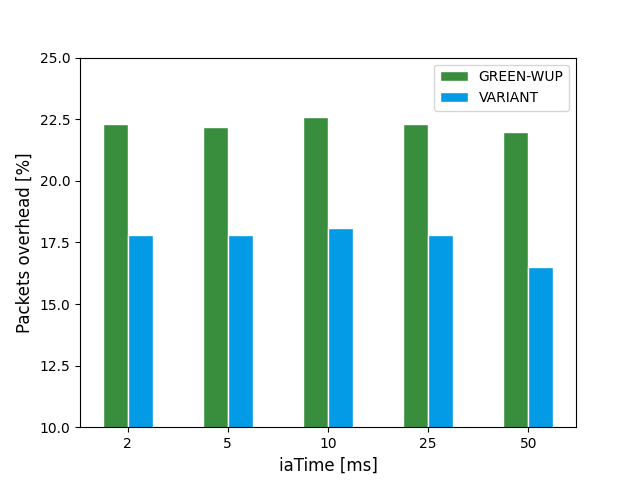
\includegraphics[width=1\linewidth]{overhead_plot.png}
        \caption*{(a)}
    \end{minipage}%
    \begin{minipage}{.5\textwidth}
        \centering
        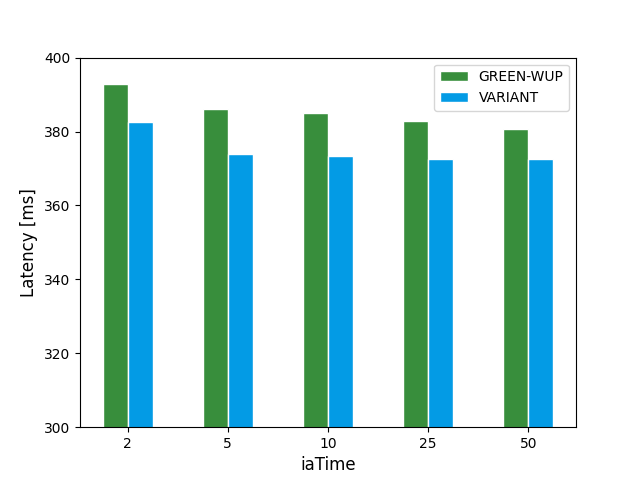
\includegraphics[width=1\linewidth]{latency_plot.png}
        \caption*{(b)}
    \end{minipage}
    \caption{Comparazione fra i due protocolli: (a) l'overhead di rete e (b) le latenze sperimentate.}
\end{figure}

Osservando la \textbf{Figura 4.1} è evidente che nella variante l'overhead diminuisce in quanto diminuisce il numero totale di pacchetti di controllo inviati
per garantire il corretto trasferimento dei pacchetti dati. Il numero di quest'ultimi scende dal 22.3\% medio richiesto dall'implementazione originale
di GREEN-WUP al 17.5\% medio richiesto dalla variante. In particolare, il numero dei pacchetti CTS inviati è di circa il 27\% in meno rispetto
al precedente approccio e ciò segue dal fatto che un minor numero di nodi viene coinvolto ad ogni step di selezione del nodo
intermedio. In altri termini, con la variante proposta si vuole ridurre allo stretto necessario il numero dei nodi coinvolti nella selezione del
\emph{relay node} e contemporaneamente evitare sprechi energetici.\\

Conseguentemente, la latenza media richiesta per far recapitare un pacchetto (DATA) al sink node è più bassa nella variante, in quanto minore il
numero di pacchetti in circolazione, ovvero nei buffer dei nodi della rete. In particolare, la fase di ricerca dei nodi viene lievemente estesa in
quanto nella variante l'insieme dei nodi candidati risulta essere ulteriormente partizionto, tuttavia questo è bilanciato dal fatto che i tempi
di selezione dei nodi disponibili (attraverso lo scambio di RTS/CTS) diminuisce, favorendo quindi latenze più basse.

\newpage

\begin{figure}
    \centering
    \begin{minipage}{.5\textwidth}
        \centering
        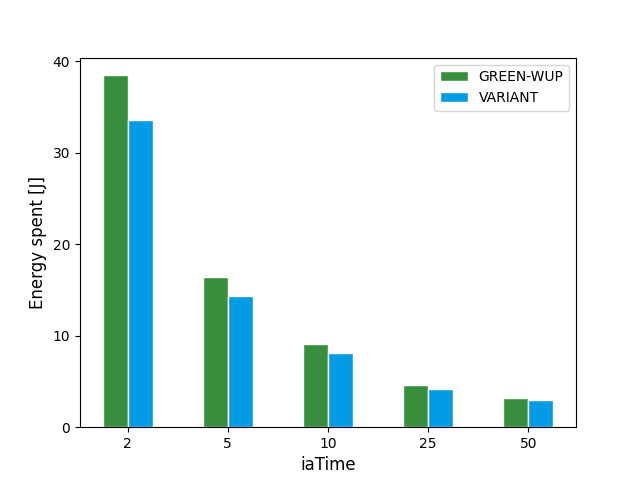
\includegraphics[width=1\linewidth]{energy_plot.png}
        \caption*{(a)}
    \end{minipage}%
    \begin{minipage}{.5\textwidth}
        \centering
        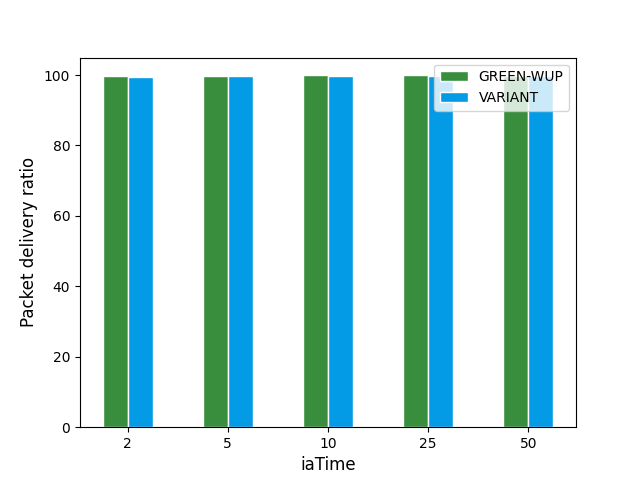
\includegraphics[width=1\linewidth]{pdr_plot.png}
        \caption*{(b)}
    \end{minipage}
    \caption{Comparazione fra i due protocolli: (a) l'energia spesa dalla rete e (b) il packet delivery ratio.}
\end{figure}

Analizzando la \textbf{Figura 4.2} si può notare come l'energia richiesta dalla rete è inferiore nel caso della variante. Come diretta conseguenza di quanto
sopra esposto i consumi energetici sono ridotti in quanto i nodi della rete rispondono alle sequenze di wake up con sematic addressing in
numero minore rispetto alla versione originale. In particolare, la massima efficienza energetica è raggiunta in condizioni di elevato stress
della rete in quanto più alta la probabilità che un maggior numero di messaggi di wake up con semantic addressing svegli i nodi candidati. In altri
termini, la rete subisce un forte aumento dei pacchetti in circolazione, e quindi di messaggi di wake up, ed in questo scenario gli effetti della
modifica che permette ai nodi di scegliere se attivare o meno la radio principale è ancor più evidente. L'efficienza energetica è favorita non solo
da questa modifica ma anche dalla stessa applicazione di jitter che vengono calcolati a partire dallo stato dei nodi
e che non sono puramente randomici come nel caso dell'implementazione originale di GREEN-WUP.

\newpage

\begin{figure}
    \centering
    \begin{minipage}{.5\textwidth}
        \centering
        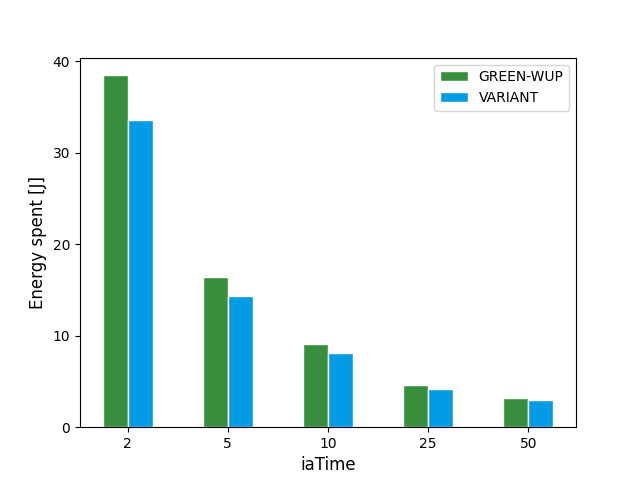
\includegraphics[width=1\linewidth]{energy_plot.png}
        \caption*{(a)}
    \end{minipage}%
    \begin{minipage}{.5\textwidth}
        \centering
        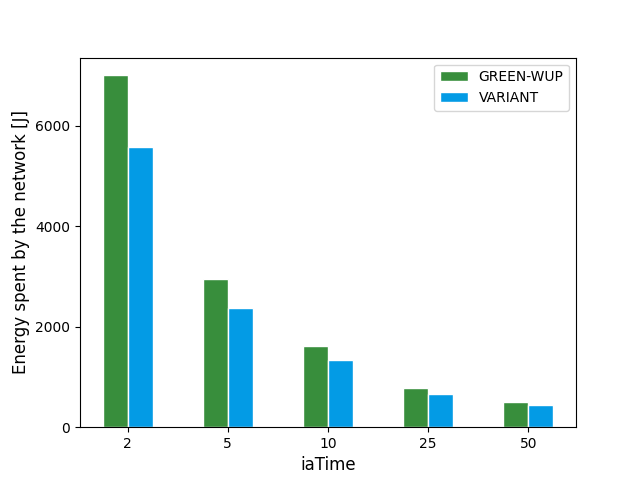
\includegraphics[width=1\linewidth]{interest_energy_plot.png}
        \caption*{(b)}
    \end{minipage}
    \caption{Comparazione energetica di GREEN-WUP e variante senza (a) e con (b) fase di interest dissemination per determinare l'hop count.}
\end{figure}

I risultati in \textbf{Figura 4.3} mostrano i costi energetici aggiuntivi richiesti implementando anche la fase di interest
dissemination sia in GREEN-WUP che nella variante. Si noti come i consumi energetici aggiuntivi possono essere considerati costanti in quanto
la fase di interest dissemination viene eseguita solo inizialmente prima della fase di scambio dati. In effetti l'overhead energetico
richiesto rimane costante sotto 1J per ciascun valore assunto da \emph{iaTime}.


\chapter{Ottimizzazione dei parametri}

\chapter{Conclusioni}

\backmatter
\cleardoublepage
\phantomsection % Give this command only if hyperref is loaded
\addcontentsline{toc}{chapter}{\bibname}

\begin{thebibliography}{9}

    \bibitem{energy-harvesting-paper}
    Stefano Basagni, Georgia Koutsandria, Chiara Petrioli.
    \textit{A Comparative Performance Evaluation of Wake-up Radio-based Data Forwarding for Green Wireless Networks}.

    \bibitem{wake-up-radios-paper}
    Stefano Basagni, Valerio Di Valerio, Georgia Koutsandria, Chiara Petrioli.
    \textit{Wake-up Radio-enabled Routing for Green Wireless Sensor Networks}
\end{thebibliography}

\end{document}